\documentclass{article}
\usepackage[margin=1in]{geometry}
\usepackage{pgf}
\usepackage{tikz}
\usetikzlibrary{arrows,automata}
\usepackage[latin1]{inputenc}
\usepackage{listings}
\lstdefinestyle{customc}{
  belowcaptionskip=1\baselineskip,
  breaklines=true,
  frame=L,
  xleftmargin=\parindent,
  language=C,
  showstringspaces=false,
  basicstyle=\footnotesize\ttfamily,
  keywordstyle=\bfseries\color{green!40!black},
  commentstyle=\itshape\color{purple!40!black},
  identifierstyle=\color{blue},
  stringstyle=\color{orange},
}
\lstset{escapechar=@,style=customc}

\begin{document}

\lstinputlisting[caption=page\_check\_references, style=customc]{src/page_check_references.c}
\newpage

\lstinputlisting[caption=shrink\_page\_list, style=customc]{src/simple_shrink_page_list.c}
\newpage

\begin{figure}
\center
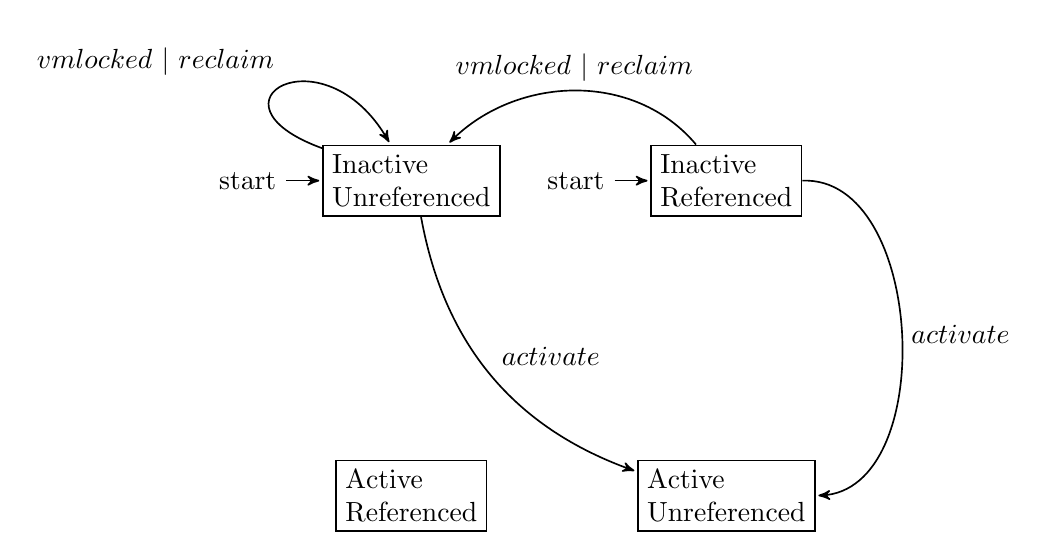
\begin{tikzpicture}[->,>=stealth',shorten >=1pt,auto,node distance=4cm,
                    semithick]

  \tikzstyle{every state}=[rectangle,draw,align=left]

  \node[initial,state] (IU)               {Inactive \\ Unreferenced};
  \node[initial,state] (IR) [right of=IU] {Inactive \\ Referenced};
  \node[state]         (AU) [below of=IR] {Active \\ Unreferenced};
  \node[state]         (AR) [below of=IU] {Active \\ Referenced};

  \path
  (IU) edge [out=160,in=120,looseness=5,align=left]      node {$vmlocked$ $\vert$ $reclaim$} (IU)
  (IR) edge [out=130,in=45,looseness=1,swap,align=left]  node {$vmlocked$ $\vert$ $reclaim$} (IU)

  (IU) edge [bend right]   node {$activate$} (AU)
  (IR) edge [bend left=90] node {$activate$} (AU)
  ;

\end{tikzpicture}
\caption{Anon LRU Automata}
\end{figure}

\begin{table}
\center
\begin{tabular}{|l|l|}
\hline
Transition & Condition                        \\
\hline
$vmlocked$ & vm\_flags \&\& VM\_LOCKED        \\
$activate$ & !vmlocked \&\&  referenced\_ptes \\
$reclaim$  & !vmlocked \&\& !referenced\_ptes \\
\hline
\end{tabular}
\caption{Anon LRU Automata Legend}
\end{table}

\begin{figure}
\center
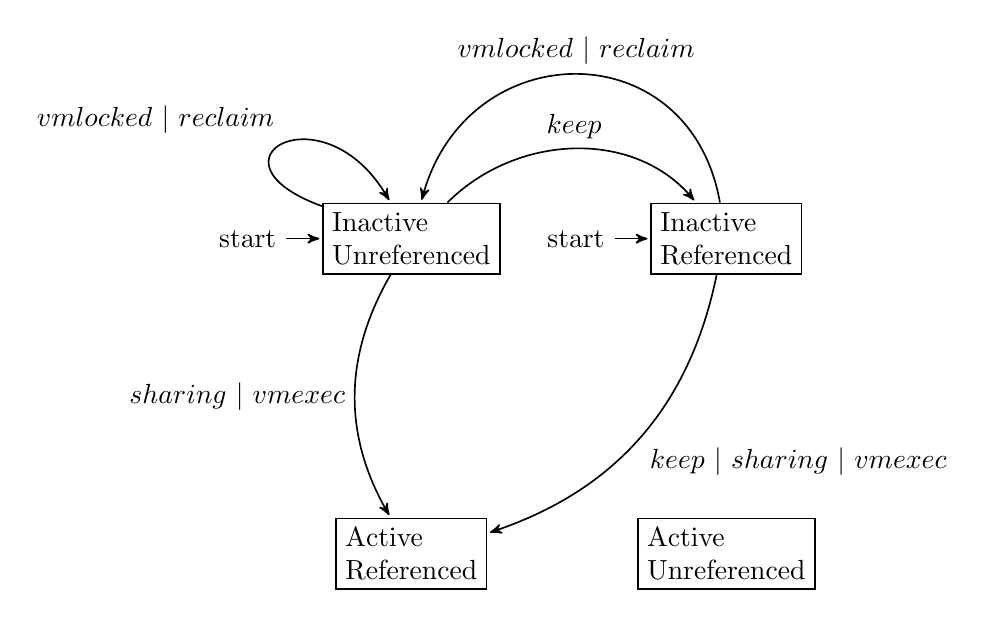
\begin{tikzpicture}[->,>=stealth',shorten >=1pt,auto,node distance=4cm,
                    semithick]

  \tikzstyle{every state}=[rectangle,draw,align=left]

  \node[initial,state] (IU)               {Inactive \\ Unreferenced};
  \node[initial,state] (IR) [right of=IU] {Inactive \\ Referenced};
  \node[state]         (AU) [below of=IR] {Active \\ Unreferenced};
  \node[state]         (AR) [below of=IU] {Active \\ Referenced};

  \path
  (IU) edge [out=160,in=120,looseness=5,align=left]       node {$vmlocked$ $\vert$ $reclaim$} (IU)
  (IR) edge [out=100,in=75,looseness=1.5,align=left,swap] node {$vmlocked$ $\vert$ $reclaim$} (IU)
  (IU) edge [in=130,out=45,looseness=1,align=left]        node {$keep$} (IR)

  (IR) edge [bend left]       node {$keep$ $\vert$ $sharing$ $\vert$ $vmexec$} (AR)
  (IU) edge [bend right,swap] node {$sharing$ $\vert$ $vmexec$} (AR)
  ;
\end{tikzpicture}
\caption{File LRU Automata}
\end{figure}

\begin{table}
\center
\begin{tabular}{|l|l|}
\hline
Transition & Condition \\
\hline
$vmlocked$ &                                       vm\_flags \&\& VM\_LOCKED  \\
$keep$     & !vmlocked \&\& referenced\_ptes                                  \\
$vmexec$   & $keep$    \&\&                        vm\_flags \&\& VM\_EXEC    \\
$sharing$  & $keep$    \&\& referenced\_ptes $>$ 1                            \\
$reclaim$  & !vmlocked \&\& !referenced\_ptes                                 \\
\hline
\end{tabular}
\caption{File LRU Automata Legend}
\end{table}

\begin{figure}
\center
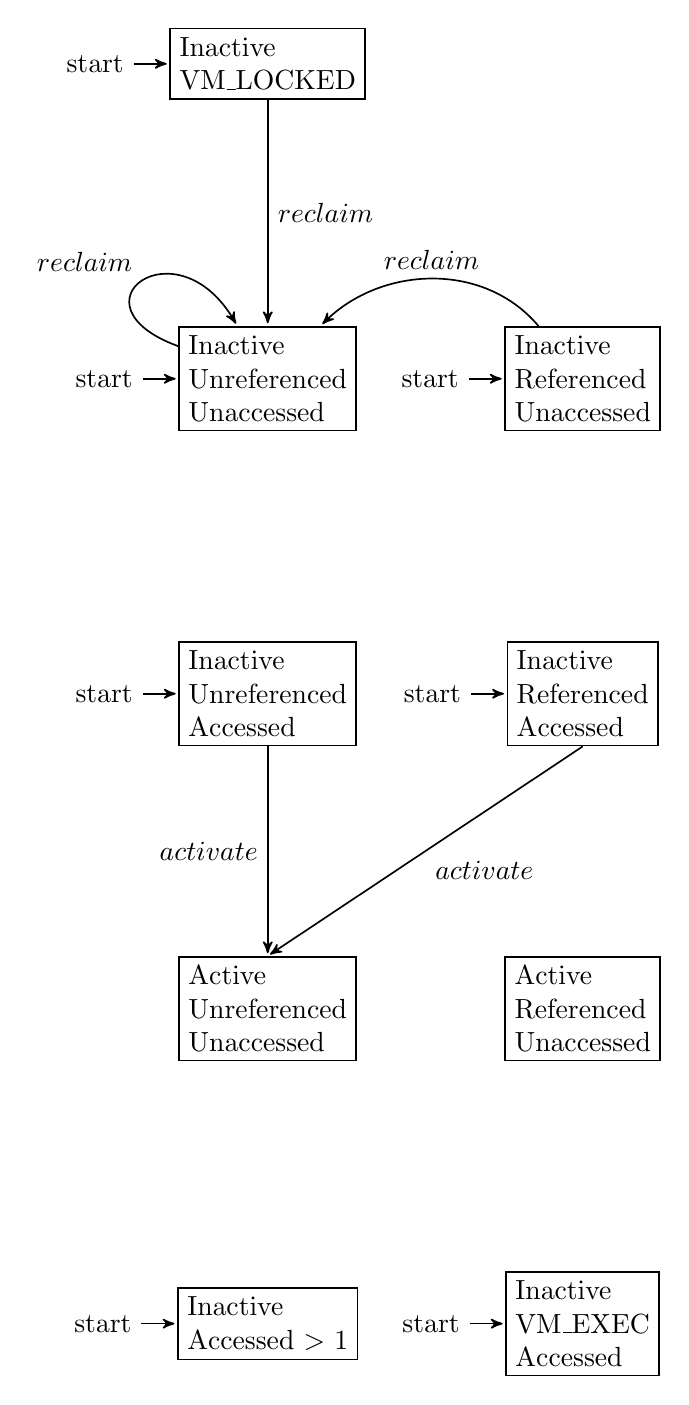
\begin{tikzpicture}[->,>=stealth',shorten >=1pt,auto,node distance=4cm,
                    semithick]

  \tikzstyle{every state}=[rectangle,draw,align=left]

  \node[initial,state] (IUU)                {Inactive \\ Unreferenced \\ Unaccessed};
  \node[initial,state] (IRU) [right of=IUU] {Inactive \\ Referenced   \\ Unaccessed};
  \node[initial,state] (LCK) [above of=IUU] {Inactive \\ VM\_LOCKED};

  \node[initial,state] (IUA) [below of=IUU] {Inactive \\ Unreferenced \\ Accessed  };
  \node[initial,state] (IRA) [right of=IUA] {Inactive \\ Referenced   \\ Accessed  };

  \node[state]         (AUU) [below of=IUA] {Active   \\ Unreferenced \\ Unaccessed};
  \node[state]         (ARU) [right of=AUU] {Active   \\ Referenced   \\ Unaccessed};

  \node[initial,state] (IAA) [below of=AUU] {Inactive \\ Accessed $>$ 1};
  \node[initial,state] (IAE) [right of=IAA] {Inactive \\ VM\_EXEC \\ Accessed};

  \path
  (LCK) edge [out=270,in=90,looseness=0]      node {$reclaim$} (IUU)
  (IUU) edge [out=160,in=120,looseness=5]     node {$reclaim$} (IUU)
  (IRU) edge [out=130,in=45,looseness=1,swap] node {$reclaim$} (IUU)

  (IUA) edge [out=270,in=90,looseness=0,swap] node {$activate$} (AUU)
  (IRA) edge [out=270,in=90,looseness=0]      node {$activate$} (AUU)
  ;
\end{tikzpicture}
\caption{Anon LRU Automata}
\end{figure}

\begin{figure}
\center
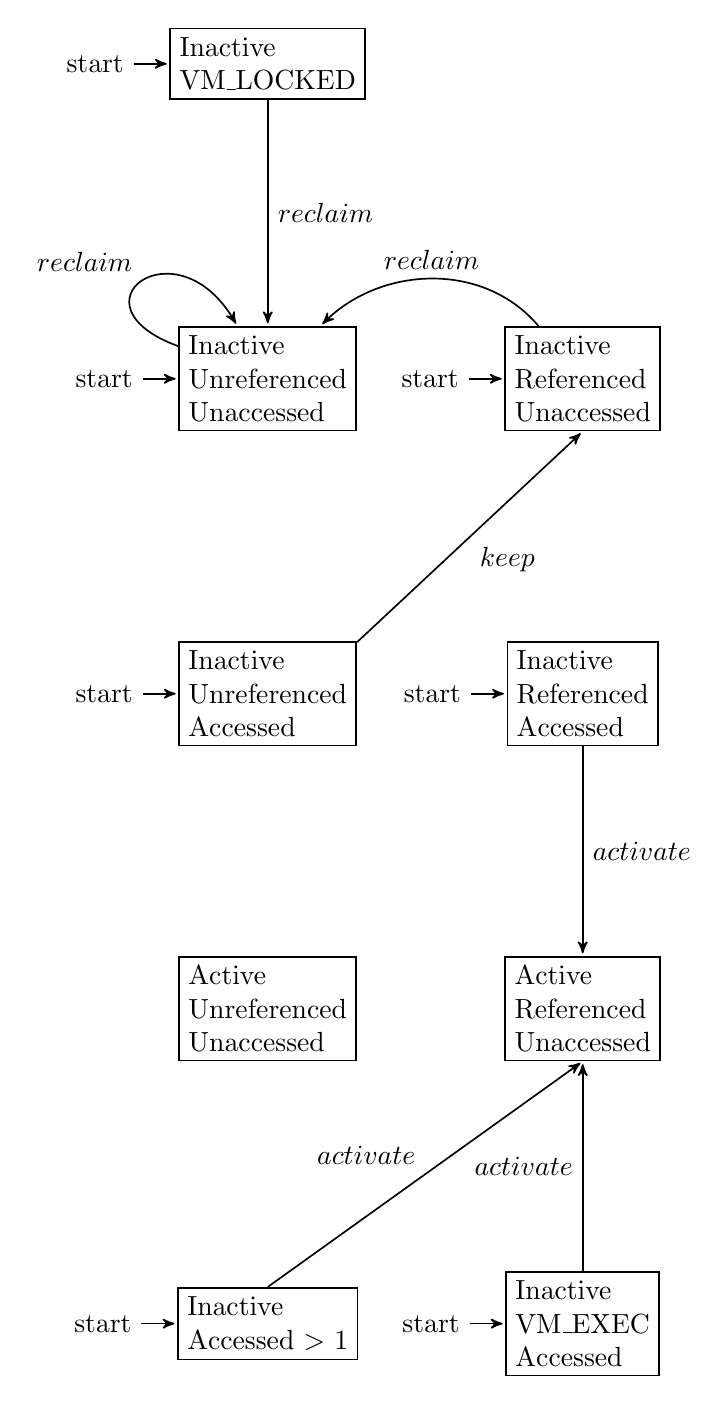
\begin{tikzpicture}[->,>=stealth',shorten >=1pt,auto,node distance=4cm,
                    semithick]

  \tikzstyle{every state}=[rectangle,draw,align=left]

  \node[initial,state] (IUU)                {Inactive \\ Unreferenced \\ Unaccessed};
  \node[initial,state] (IRU) [right of=IUU] {Inactive \\ Referenced   \\ Unaccessed};
  \node[initial,state] (LCK) [above of=IUU] {Inactive \\ VM\_LOCKED};

  \node[initial,state] (IUA) [below of=IUU] {Inactive \\ Unreferenced \\ Accessed  };
  \node[initial,state] (IRA) [right of=IUA] {Inactive \\ Referenced   \\ Accessed  };

  \node[state]         (AUU) [below of=IUA] {Active   \\ Unreferenced \\ Unaccessed};
  \node[state]         (ARU) [right of=AUU] {Active   \\ Referenced   \\ Unaccessed};

  \node[initial,state] (IAA) [below of=AUU] {Inactive \\ Accessed $>$ 1};
  \node[initial,state] (IAE) [right of=IAA] {Inactive \\ VM\_EXEC \\ Accessed};


  \path
  (LCK) edge [out=270,in=90,looseness=0]      node {$reclaim$} (IUU)
  (IUU) edge [out=160,in=120,looseness=5]     node {$reclaim$} (IUU)
  (IRU) edge [out=130,in=45,looseness=1,swap] node {$reclaim$} (IUU)

  (IUA) edge [in=270,out=30,looseness=0,swap] node {$keep$} (IRU)
  (IRA) edge [out=270,in=90,looseness=0]      node {$activate$} (ARU)

  (IAA) edge [out=90,in=270,looseness=0] node {$activate$} (ARU)
  (IAE) edge [out=90,in=270,looseness=0] node {$activate$} (ARU)
  ;
\end{tikzpicture}
\caption{File LRU Automata}
\end{figure}

\end{document}
